\documentclass[https://www.overleaf.com/project/63761df255a8a9f4a15c3579
	letterpaper, % Paper size, specify a4paper (A4) or letterpaper (US letter)
	10pt, % Default font size, specify 10pt, 11pt or 12pt
]{CSUniSchoolLabReport}


\usepackage{verbatim}
\usepackage{fontawesome}
\usepackage{hyperref}
\usepackage[normalem]{ulem}
\usepackage{listings}
\usepackage{xcolor}
\definecolor{codegreen}{rgb}{0,0.6,0}
\definecolor{codegray}{rgb}{0.5,0.5,0.5}
\definecolor{codepurple}{rgb}{0.58,0,0.82}
\definecolor{backcolour}{rgb}{1,1,1}
\lstdefinestyle{mystyle}{
    backgroundcolor=\color{backcolour},   
    commentstyle=\color{codegreen},
    keywordstyle=\color{magenta},
    numberstyle=\tiny\color{codegray},
    stringstyle=\color{codepurple},
    basicstyle=\ttfamily\footnotesize,
    breakatwhitespace=false,         
    breaklines=true,                 
    captionpos=b,                    
    keepspaces=true,                 
    numbers=left,                    
    numbersep=5pt,                  
    showspaces=false,                
    showstringspaces=false,
    showtabs=false,                  
    tabsize=2
}

\lstset{style=mystyle}
\renewcommand\ULthickness{1.0pt}   %%---> For changing thickness of underline
\setlength\ULdepth{1.3ex}%\maxdimen ---> For changing depth of underline

%----------------------------------------------------------------------------------------
%	REPORT INFORMATION
%----------------------------------------------------------------------------------------


\begin{document}
    
    \begin{figure}[H] % [H] forces the figure to be placed exactly where it appears in the text
    	\centering % Horizontally center the figure
    	
\includegraphics[width=0.4\textwidth]{images/logo.png} % Include the figure
    \end{figure}
    
    \begin{center}
        \begin{tabular} {c}
            \Huge Universidad La Salle \\\\\\\\
            \huge Construcción de Software \\\\\\\\
            \LARGE Informe \\\\\\\\
            \huge Familia de normas ISO/IEC 25000 \\\\\\\\
            \LARGE Karlo Emigdio Pacha Curimayhua \\\\\\\\
            \LARGE Séptimo Semestre - Ingeniería de Software \\\\\\\\
            \LARGE 2023
          \end{tabular}
    \end{center}
    
    \begin{center}
    	\begin{tabular}{l r}
    	\end{tabular}
    \end{center}
    
    %----------------------------------------------------------------------------------------
    %	Introducción
    %----------------------------------------------------------------------------------------
    
    \section{Introducción }
    
        La calidad del software es un factor clave para el éxito de las organizaciones, especialmente ahora que la tecnología controla y opera en todos los campos. Los productos software de alta calidad son más fáciles de usar, más seguros y más eficientes; también son más rentables de desarrollar y mantener.
        \\\\
        En un mundo cada vez más digital, los productos software son una parte esencial de nuestras vidas; es por eso que es importante que las organizaciones se aseguren de que sus productos software cumplan con los requisitos de calidad de sus clientes y usuarios.
        \\
        Las normas ISO/IEC 25000 son una herramienta valiosa para las organizaciones que desean cumplir con los requisitos de calidad de sus productos software. Estas normas proporcionan un marco de trabajo sólido que puede ayudar a las organizaciones a comprender y mejorar la calidad de sus productos software.
        \\\\
        El objetivo de las normas ISO/IEC 25000 es proporcionar un marco de trabajo para la evaluación de la calidad del producto software. Estas normas están diseñadas para ayudar a las organizaciones a cumplir con los requisitos de calidad de sus productos software.
        
    %----------------------------------------------------------------------------------------
    %	Historia
    %----------------------------------------------------------------------------------------
    
    \section{Historia}
        La familia de normas ISO/IEC 25000 es un conjunto de normas internacionales que proporcionan un marco de trabajo para la evaluación de la calidad del producto software. Estas normas están diseñadas para ayudar a las organizaciones a comprender y mejorar la calidad de sus productos software.
        \\
        La historia de la familia de normas ISO/IEC 25000 se remonta a la década de 1980, cuando se desarrollaron las primeras normas sobre la calidad del producto software. En 1992, la Organización Internacional de Normalización (ISO) y la Comisión Electrotécnica Internacional (IEC) publicaron la norma ISO/IEC 9126, que define un modelo de calidad del producto software. 
        \\\\
        En 1998, ISO publicó la norma ISO/IEC 14598, que abordaba el proceso de evaluación de la calidad del producto software.
        \\
        En 2005, ISO y IEC comenzaron a trabajar en una nueva familia de normas sobre la calidad del producto software. Esta familia de normas se conoce como ISO/IEC 25000, también conocida como SQuaRE (System and Software Quality Requirements and Evaluation), es una familia de normas que tiene por objetivo la creación de un marco de trabajo común para evaluar la calidad del producto software.
        \\\\
        La familia ISO/IEC 25000 es el resultado de la evolución de otras normas anteriores, especialmente de las normas ISO/IEC 9126, que describe las particularidades de un modelo de calidad del producto software, e ISO/IEC 14598, que abordaba el proceso de evaluación de productos software. 
        \\
        La creación del estándar ISO/IEC 25000 tiene como objetivo organizar, enriquecer y unificar las series que cubren dos procesos principales: especificación de requisitos de calidad del software y evaluación de la calidad del software, soportada por el proceso de medición de calidad del software.
    
    \subsection{Divisiones}
        La familia ISO/IEC 25000 se encuentra compuesta por cinco divisiones.

        \subsection*{2.1.1 \hspace{0.5em} SO/IEC 2500n – División de Gestión de Calidad}
            Las normas que forman esta división definen todos los modelos, términos y definiciones comunes referenciados por todas las otras normas de la familia ISO/IEC 25000.  Esta división está compuesta por:
            \\\\
            - ISO/IEC 25000 - Guide to SQuaRE.
            \\
            - ISO/IEC 25001 - Planning and Management.

        \subsection*{2.1.2 \hspace{0.5em} ISO/IEC 2501n – División de Modelo de Calidad}
            Las normas de esta división presentan modelos de calidad detallados, incluyendo características para calidad interna, externa y en uso del producto software. Esta división está compuesta por:
            \\\\
            - ISO/IEC 25010 - System and software quality models.
            \\
            - ISO/IEC 25012 - Data Quality model.

        \subsection*{2.1.3 \hspace{0.5em} ISO/IEC 2502n – División de Medición de Calidad}
            Las normas de esta división incluyen un modelo de referencia de la medición de la calidad del producto, definiciones de medidas de calidad (interna, externa y en uso) y guías prácticas para su aplicación. Esta división está compuesta por:
            \\\\
            - ISO/IEC 25020 - Measurement reference model and guide.
            \\
            - ISO/IEC 25021 - Quality measure elements.
            \\
            - ISO/IEC 25022 - Measurement of quality in use.
            \\
            - ISO/IEC 25023 - Measurement of system and software product quality.
            \\
            - ISO/IEC 25024 - Measurement of data quality.

        \subsection*{2.1.4 \hspace{0.5em} ISO/IEC 2503n – División de Requisitos de Calidad}
            Las normas de esta división ayudan a especificar requisitos de calidad que pueden ser utilizados en el proceso de elicitación de requisitos de calidad del producto software a desarrollar o como entrada del proceso de evaluación. Esta división está compuesta por:
            \\\\
            - ISO/IEC 25030 - Quality requirements.

        \subsection*{2.1.5 \hspace{0.5em} ISO/IEC 2504n – División de Evaluación de Calidad}
            Esta división incluye normas que proporcionan requisitos, recomendaciones y guías para llevar a cabo el proceso de evaluación del producto software. Esta división está compuesta por:
            \\\\
            - ISO/IEC 25040 - Evaluation reference model and guide.
            \\
            - ISO/IEC 25041 - Evaluation guide for developers, acquirers and independent evaluators.
            \\
            - ISO/IEC 25042 - Evaluation modules.
            \\
            - ISO/IEC 25045 - Evaluation module for recoverability.

        \begin{center}
            \begin{tabular}{| c | c |}
                \hline
                   ISO/IEC & Año de publicación\\ 
                \hline
                    25000 & 2005\\
                    25001 & 2007\\
                    25010 & 2011\\
                    25012 & 2008\\
                    25020 & 2007\\
                    25021 & 2007\\
                    25030 & 2007\\
                    25051 & 2006\\
                    25062 & 2006\\
                \hline
            \end{tabular}
        \end{center}
        
        \begin{center}
            \textbf{Tabla 1.}\hspace{0.5em} Año de publicación de las versiones ISO/IEC 25000. Fuente: Wikipedia.
        \end{center}

    \subsection{Versiones}

        \subsection*{2.2.1 \hspace{0.5em} ISO/IEC 25000:}
            Contiene el modelo de la arquitectura de SQuaRE, un resumen de las partes, los usuarios previstos y las partes asociadas, así como los modelos de referencia.

        \subsection*{2.2.2 \hspace{0.5em} ISO/IEC 25001:}
            Establece los requisitos y orientaciones para gestionar la evaluación y especificación de los requisitos del producto software.
            
        \subsection*{2.2.3 \hspace{0.5em} ISO/IEC 25010:}
        Describe el modelo de calidad para el producto software y para la calidad en uso. Esta Norma presenta las características y sub características de calidad frente a las cuales evaluar el producto software.
            
        \subsection*{2.2.4 \hspace{0.5em} ISO/IEC 25012:}
            Define un modelo general para la calidad de los datos, aplicable a aquellos datos que se encuentran almacenados de manera estructurada y forman parte de un Sistema de Información.
            
        \subsection*{2.2.5 \hspace{0.5em} ISO/IEC 25020:}
            Presenta una explicación introductoria y un modelo de referencia común a los elementos de medición de la calidad. También proporciona una guía para que los usuarios seleccionen o desarrollen y apliquen medidas propuestas por normas ISO.
            
        \subsection*{2.2.6 \hspace{0.5em} ISO/IEC 25021:}
            Define y especifica un conjunto recomendado de métricas base y derivadas que puedan ser usadas a lo largo de todo el ciclo de vida del desarrollo software.
            
        \subsection*{2.2.7 \hspace{0.5em} ISO/IEC 25022:}
            Define específicamente las métricas para realizar la medición de la calidad en uso del producto.
            
        \subsection*{2.2.8 \hspace{0.5em} ISO/IEC 25023:}
            Define específicamente las métricas para realizar la medición de la calidad de productos y sistemas software.
            
        \subsection*{2.2.9 \hspace{0.5em} ISO/IEC 25024:}
            Define específicamente las métricas para realizar la medición de la calidad de datos.
            
        \subsection*{2.2.10 \hspace{0.5em} ISO/IEC 25030:} 
            Provee de un conjunto de recomendaciones para realizar la especificación de los requisitos de calidad del producto software.
            
        \subsection*{2.2.11 \hspace{0.5em} ISO/IEC 25040:} 
            Propone un modelo de referencia general para la evaluación, que considera las entradas al proceso de evaluación, las restricciones y los recursos necesarios para obtener las correspondientes salidas.
            
        \subsection*{2.2.12 \hspace{0.5em} ISO/IEC 25041:} 
            Describe los requisitos y recomendaciones para la implementación práctica de la evaluación del producto software desde el punto de vista de los desarrolladores, de los adquirentes y de los evaluadores independientes.
            
        \subsection*{2.2.13 \hspace{0.5em} ISO/IEC 25042:}
            Define lo que la Norma considera un módulo de evaluación y la documentación, estructura y contenido que se debe utilizar a la hora de definir uno de estos módulos.
            
        \subsection*{2.2.14 \hspace{0.5em} ISO/IEC 25045:}
            Define un módulo para la evaluación de la subcaracterística Recuperabilidad.
            
        \subsection*{2.2.15 \hspace{0.5em} ISO/IEC 25059:}
            Extiende las características del modelo de calidad de la norma ISO/IEC 25010 para incluir aspectos adicionales que se presentan en sistemas de inteligencia artificial.
            \\\\
            - Adecuación Funcional: Adaptabilidad Funcional.
            \\
            - Usabilidad: Controlabilidad del Usuario, y Transparencia.
            \\
            - Fiabilidad: Robustez.
            \\
            - Seguridad: Intervenibilidad.



    %----------------------------------------------------------------------------------------
    %	Características
    %----------------------------------------------------------------------------------------
    
    \section{Características}
        \subsection*{3.1 \hspace{0.5em} Adecuación Funcional (funcionalidad) }
            Capacidad para proporcionar funciones que satisfagan las necesidades declaradas e implícitas.
            \\\\
            -Idoneidad
            \\
            -Precisión
            \\
            -Interoperabilidad
            \\
            -Seguridad
            \\
            -Cumplimiento de la funcionalidad

        \subsection*{3.2 \hspace{0.5em} Fiabilidad}
            Capacidad para desempeñar las funciones específicas (uso en condiciones y tiempo determinados).
            \\\\
            - Madurez
            \\
            - Tolerancia a fallos
            \\
            - Recuperabilidad
            \\
            - Cumplimiento de fiabilidad

        \subsection*{3.3 \hspace{0.5em} Usabilidad}
            Capacidad de ser entendido, aprendido, usado y resultar atractivo para el usuario.
            \\\\
            - Inteligibilidad
            \\
            - Facilidad de aprendizaje
            \\
            - Operabilidad
            \\
            - Atractividad
            \\
            - Cumplimiento de usabilidad

        \subsection*{3.4 \hspace{0.5em} Eficiencia}
            Capacidad de desempeñarse, realizar o cumplir adecuadamente una función en relación con los recursos.
            \\\\
            - Utilización de los recursos
            \\
            - Comportamiento en el tiempo
            \\
            - Cumplimiento de la eficiencia

        \subsection*{3.5 \hspace{0.5em} Mantenibilidad}
            Capacidad para ser modificado efectivamente y eficientemente.
            \\\\
            - Analizabilidad
            \\
            - Cambiabilidad
            \\
            - Estabilidad
            \\
            - Capacidad de ser probado
            \\
            - Cumplimiento de mantenibilidad

        \subsection*{3.6 \hspace{0.5em} Portabilidad}
            Capacidad de ser transferido de forma efectiva y eficiente de un entorno hardware o software.
            \\\\
            - Adaptabilidad
            \\
            - Facilidad de instalación
            \\
            - Coexistencia
            \\
            - Intercambiabilidad
            \\
            - Cumplimiento de portabilidad
        \\\\
        Las características cambian según la versión de la norma ISO/IEC 25000 en la que se esté trabajando.

        \begin{center}
            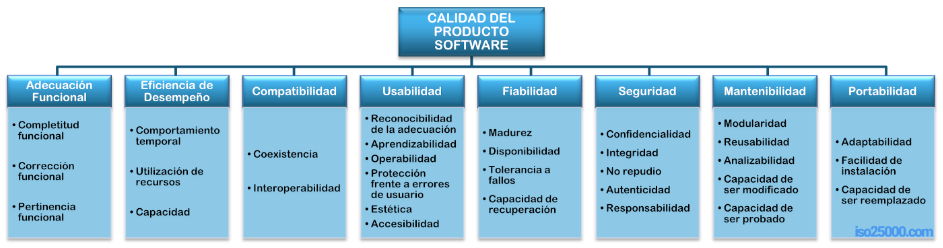
\includegraphics[width=1.0\linewidth]{image.png}
        \end{center}
        \begin{center}
            \textbf{Figura 1.}\hspace{0.5em} Características según las normas ISO/IEC 25010.
        \end{center}

        \begin{center}
            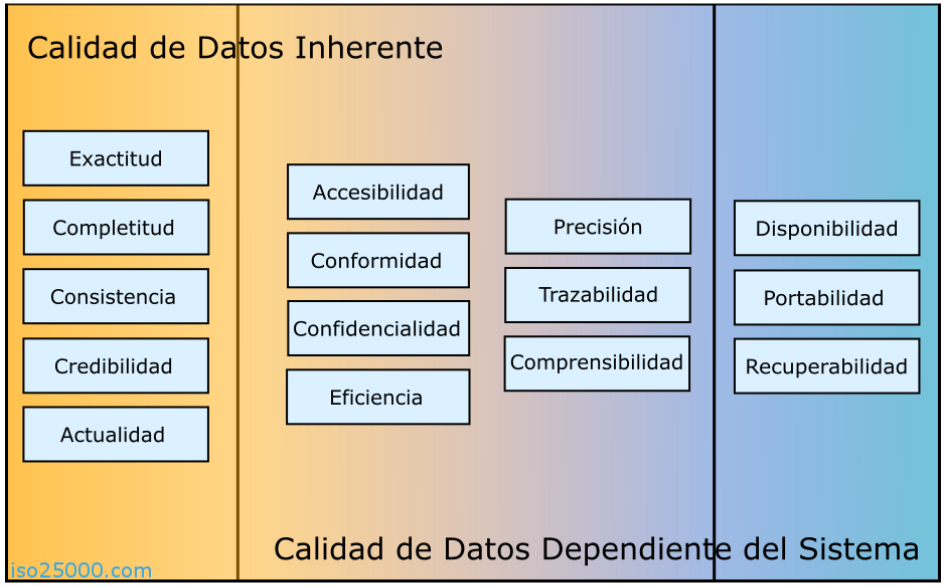
\includegraphics[width=1\linewidth]{image2.png}
        \end{center}
        \begin{center}
            \textbf{Figura 2.}\hspace{0.5em} Características según las normas ISO/IEC 25012.
        \end{center}

    %----------------------------------------------------------------------------------------
    %	Caso de Estudio
    %----------------------------------------------------------------------------------------
    
    \section{Caso de Estudio}
        En el trabajo de Ramos entre otros [5], se evaluaron las soluciones de correo electrónico Outlook Web Access (OWA) y Thunderbird para una institución gubernamental real. Se utilizaron las normas ISO/IEC 25000 para evaluar la calidad de los requisitos del software y la calidad del software en sí. 
        \\
        El estudio se centró en las características técnicas y funcionales de ambas soluciones, como la asistencia para configurar cuentas de correo electrónico, la libreta de direcciones, el archivo de mensajes, la privacidad sólida, la protección contra la suplantación de identidad, la actualización automática, la eliminación de basura, la integración con Exchange y la gestión de carpetas para hacer una copia de seguridad de la información. 
        \\\\
        Este trabajo proporciona un interesante caso de estudio de la implementación de las normas ISO/IEC 25000 en una institución gubernamental y detalla sus beneficios como método para evaluar la calidad del software.
        \\\\
        El modelo de referencia general se creó para ayudar a los usuarios a navegar a través de los diferentes estándares de SQuaRE (Figura 3). La elección de los estándares adecuados y los documentos de la serie SQuaRE depende del rol del usuario y de sus necesidades de información.

        \begin{center}
            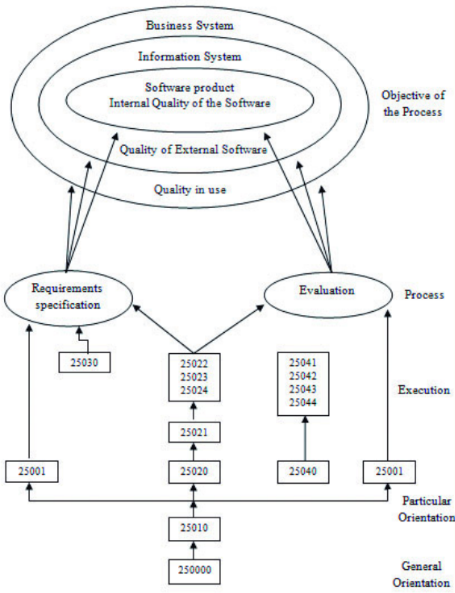
\includegraphics[width=1\linewidth]{image3.png}
        \end{center}
        \begin{center}
            \textbf{Figura 3.}\hspace{0.5em} Aplicación del Modelo SQuaRE.
        \end{center}

        \subsection{Ejecución de las actividades}
            \subsection*{4.1.1 \hspace{0.5em} Establecimiento de requisitos de evaluación}
                El proceso de evaluación se lleva a cabo para:
                \\\\
                - Comprender y evaluar los efectos positivos y negativos del producto cuando está en uso.
                \\
                - Garantizar la calidad del producto de software.
                \\
                - Medir el software desde una perspectiva técnica y funcional.
                \\
                - Proporcionar seguridad de la información.
            
            \subsection*{4.1.2 \hspace{0.5em} Identificación de las partes del producto a incluir en el proceso de evaluación}
                - Especificaciones del producto
                \\
                - Producto durante su ejecución
                \\
                - Resultados de la prueba

        \subsection{Especificación de la Evaluación}
            \subsection*{4.2.1 \hspace{0.5em} Selección de módulos de evaluación}
                Las métricas utilizadas para evaluar la calidad interna y externa del producto de software fueron: 
                \\\\
                - Adecuación funcional
                \\
                - Fiabilidad
                \\
                - Eficiencia del rendimiento
                \\
                - Usabilidad
                \\
                - Seguridad
                \\
                - Compatibilidad
                \\
                - Mantenibilidad
                \\
                - Portabilidad
                \\\\
                Las métricas utilizadas para la calidad en uso del producto de software fueron:
                \\\\
                - Efectividad
                \\
                - Eficiencia
                \\
                - Satisfacción
                \\
                - Libertad de riesgos
                \\
                - Cobertura de contexto
            
            \subsection*{4.2.2 \hspace{0.5em} Definición de los criterios de decisión para las métricas de OWA y Thunderbird}
                Esta parte define los criterios de decisión para las métricas seleccionadas. Estos son umbrales representados por H (Alto), M (Medio), L (Bajo) y N/A (No aplicable), lo que indica el nivel de importancia de los requisitos de calidad.
                \\
                
               \begin{center}
                    \begin{tabular}{| c | c | c |}
                        \hline
                          Importancia & Símbolo & Significado\\ 
                        \hline
                            Alto & H & Debe ser evaluado\\
                            Medio & M & Se puede evaluar (no es obligatorio)\\
                            Bajo & L & No será evaluado\\
                            No aplicable & N/A & No aplica\\
                        \hline
                    \end{tabular}
                \end{center}
                
                \begin{center}
                    \textbf{Tabla 2.}\hspace{0.5em} Criterios de decisión de métricas.
                \end{center}

                \begin{center}
                    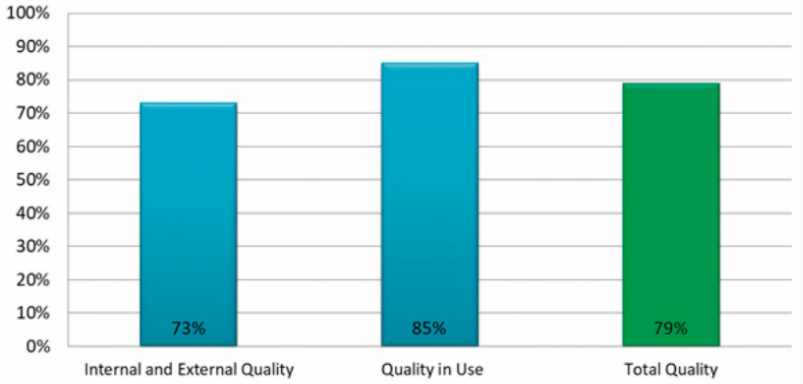
\includegraphics[width=1\linewidth]{image4.png}
                \end{center}
                \begin{center}
                    \textbf{Figura 4.}\hspace{0.5em} Resultados de calidad de OWA.
                \end{center}

                \begin{center}
                    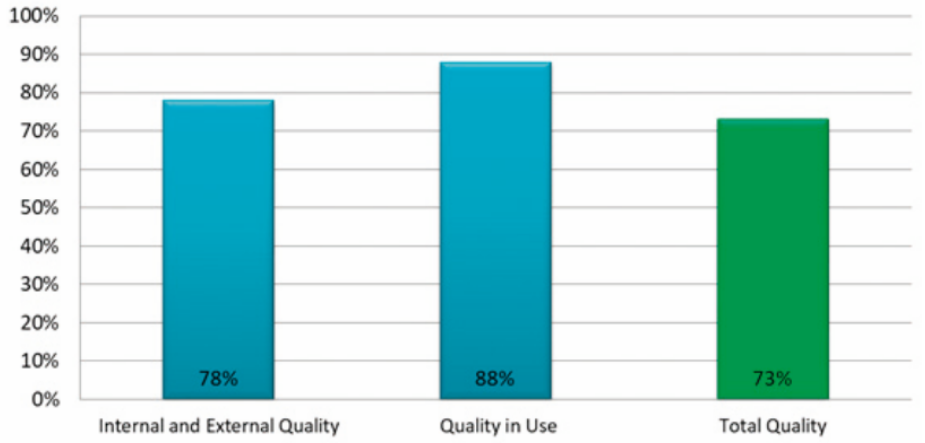
\includegraphics[width=1\linewidth]{image5.png}
                \end{center}
                \begin{center}
                    \textbf{Figura 5.}\hspace{0.5em} Resultados de calidad de Thunderbird.
                \end{center}

    
    %----------------------------------------------------------------------------------------
    %	Conclusiones
    %----------------------------------------------------------------------------------------
    
    \section{Conclusiones}
    
    En conclusión, la familia de normas ISO/IEC 25000 es una herramienta valiosa para las organizaciones que desean mejorar la calidad de sus productos software. Estas normas proporcionan un marco de trabajo holístico, adaptable y flexible que puede aplicarse a cualquier tipo de producto software. 
    \\
    Las organizaciones que desean mejorar la calidad de sus productos software deben considerar la adopción de las normas ISO/IEC 25000. Estas normas pueden ayudar a las organizaciones a desarrollar productos software de alta calidad que satisfagan las necesidades de sus clientes y usuarios.
    
    %----------------------------------------------------------------------------------------
    %	Referencias
    %----------------------------------------------------------------------------------------
    
    \section{Referencias}
        \textbf{[1]}\hspace{0.5em} Organización Internacional de Normalización (2023) Wikipedia. Disponible en: https://es.wikipedia.org/wiki/Organizaci\%C3\%B3n_Internacional_de_Normalizaci\%C3\%B3n (Accedido: 23 de octubre 2023).
        \\
        \textbf{[2]}\hspace{0.5em} ISO/IEC 25000 (2023) Wikipedia. Disponible en: https://es.wikipedia.org/wiki/ISO/IEC_25000 (Accedido: 23 octubre 2023).
        \\
        \textbf{[3]}\hspace{0.5em} Portal ISO 25000 (no date) iso25000.com. Disponible en: https://iso25000.com/index.php/normas-iso-25000/iso-25010/17-espanol (Accedido: 23 de octubre  2023).
        \\
        \textbf{[4]}\hspace{0.5em} Tema 7 - Norma ISO 9126-25000 (2020). YouTube. 7 de noviembre. Disponible en: https://www.youtube.com/watch?v=otgH3PAzzgQ (Accedido: 24 de octubre 2023).
        \\
        \textbf{[5]}\hspace{0.5em} Ramos, R.C. entre otros. (2018) “Software quality assessment applied for the governmental organizations using ISO/IEC 25000”, 2018 International Conference on eDemocracy & eGovernment (ICEDEG). doi:10.1109/icedeg.2018.8372327.\\\\

    
    %----------------------------------------------------------------------------------------
    \href{https://github.com/DAOBLUR/SoftwareConstruction/tree/main/tasks/2} {\huge\faGithub \textbf{{Repositorio GitHub}} }
    
\end{document}